% vim: spelllang=en
\documentclass[a4paper,12pt,english,parskip=half,english]{scrartcl}

\usepackage[utf8]{inputenc}
\usepackage[T1]{fontenc}
\usepackage[]{babel}
% hyphenation
\hyphenation{SoapUI Abstract-Option Abstract-Plugin SOAP-Action name-space name-spaces theo-reti-cally Content-Element}

\usepackage{subfiles}

\usepackage{url}
\usepackage{todonotes}
\presetkeys{todonotes}{inline}{}

% graphics
\usepackage{float}
\usepackage{xcolor}
% \usepackage{tikz}
% \usetikzlibrary{trees,positioning,shapes,shadows,arrows,snakes,mindmap}

% Math stuff
\usepackage{amsmath,amssymb,amsthm,wasysym}
\newcommand{\A}{\ensuremath{\mathcal{A}}}
\newcommand{\B}{\ensuremath{\mathcal{B}}}
\newcommand{\C}{\ensuremath{\mathcal{C}}}
\newcommand{\D}{\ensuremath{\mathcal{D}}}
\newcommand{\E}{\ensuremath{\mathcal{E}}}
\newcommand{\F}{\ensuremath{\mathcal{F}}}
\renewcommand{\L}{\ensuremath{\mathcal{L}}}
\newcommand{\M}{\ensuremath{\mathcal{M}}}
\newcommand{\N}{\ensuremath{\mathcal{N}}}
\renewcommand{\O}{\ensuremath{\mathcal{O}}}
\renewcommand{\P}{\ensuremath{\mathcal{P}}}
\newcommand{\R}{\ensuremath{\mathcal{R}}}
\renewcommand{\S}{\ensuremath{\mathcal{S}}}
\newcommand{\V}{\ensuremath{\mathcal{V}}}
\newcommand{\W}{\ensuremath{\mathcal{W}}}
\newcommand{\Z}{\ensuremath{\mathcal{Z}}}

% AF custom userpackeges
\usepackage{enumitem}
\usepackage{lscape}

% zeilenabstand
% \usepackage[onehalfspacing]{setspace}
\usepackage{setspace}

% section auf neuer seite beginnen
\newcommand{\mysection}{}
\let\mysection=\section
\renewcommand{\section}{\pagebreak[4]\mysection}

% compact list
\usepackage[pointedenum]{paralist}
\renewenvironment{itemize}{\begin{compactitem}}{\end{compactitem}}
\renewenvironment{enumerate}{\begin{compactenum}}{\end{compactenum}}
\renewenvironment{description}{\begin{compactdesc}}{\end{compactdesc}}
\setdefaultitem{\textbullet}{\normalfont\bfseries \textendash}{\textasteriskcentered}{\textperiodcentered}
\setdefaultitem{$\triangleright$}{$\to$}{\textbullet}{\normalfont\bfseries \textendash}

% quotation
\usepackage[babel]{csquotes}

% Use Listing
\usepackage{listings}
\lstset{language=xml,
  numbers=left,
  breaklines=true,
  prebreak=\mbox{\ {$\curvearrowright$}},
  lineskip=-0.1ex,
  frame=tlRB,
  showspaces=false,
    captionpos=b,
}

% bibtex
\usepackage[numbers,round]{natbib}
\usepackage[english]{isodate}

% header and footer
\usepackage[headsepline,footsepline]{scrpage2}
\usepackage{lastpage}

% load hyperref always as a last package
\usepackage{hyperref}

\clearscrheadfoot
\pagestyle{scrheadings}
%\automark[chapter]{section}
\automark[subsection]{section}
\renewcommand{\sectionmark}[1]{\markboth{#1}{}}%
\renewcommand{\subsectionmark}[1]{\markright{\subsectionmarkformat #1}}

% Header
\newcommand{\myihead}{\rightmark}
\newcommand{\myohead}{\leftmark}
\ihead[]{\myihead}
\ohead[]{\myohead}
%Fusszeile
\newcommand{\myifoot}{}
\newcommand{\myofoot}{\pagemark / \pageref{LastPage}}
\ifoot[]{\myifoot}
\ofoot[]{\myofoot}

\subject{Web Security Attacker Framework}
\title{WS-Attacker}
\subtitle{Documentation}
\author{Christian Mainka \and Juraj Somorovsky \and Andreas Falkenberg}
\date{\today}


\begin{document}
\maketitle

\begin{abstract}
    WS-Attacker is a modular framework for web services penetration testing. It is a free and easy to use software solution, which provides an all-in-one security checking interface with only a few clicks.

\end{abstract}

\tableofcontents

\section{How to use WS-Attacker}
\label{sec:how_to_use_ws_attacker}

This guide will use WS-Attacker for penetration testing on self-made Web Service.
The tool is based on the Paper \emph{Penetration Testing Tool for Web Services Security} presented on SERVICES 2012~\cite{MaSoSchPTT2012}.
In general, you have to to four things:

\begin{enumerate}
    \item Loading the WSDL and set up the request parameters.
    \item Submitting a test request.
    \item Configuring the attack plugins.
    \item Starting the attacks.
\end{enumerate}

\subsection{Loading a WSDL}
\label{sec:loading_a_wsdl}

After starting WS-Attacker, the GUI appears and offers an input field to enter the location
of the WSDL, see Figure \ref{fig:load_wsdl}.

\begin{figure}[h!]
    \begin{center}
        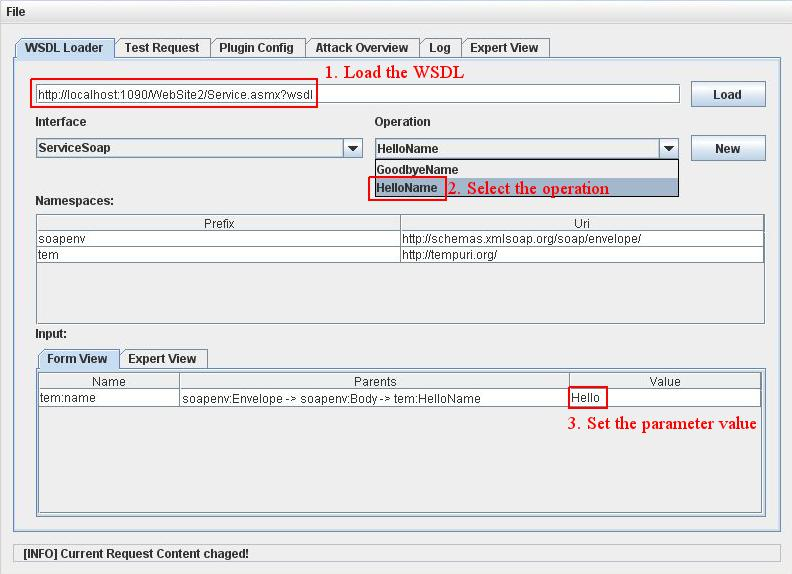
\includegraphics[width=0.8\textwidth]{img/load_wsdl}
    \end{center}
    \caption{Loading the WSDL.}
    \label{fig:load_wsdl}
\end{figure}

The custom service has two operations: \emph{HelloName} and \emph{GoodbyeName}.
\emph{HelloName} is chosen as the operation to be tested. The table at the bottom gives a
form based input possibility for all request parameters and in this case, \emph{name} is set to
\emph{Hello}.

\subsection{Submitting a Test Request}
\label{sec:submitting_a_test_request}

Next step is to do a test request: Figure \ref{fig:test_request} shows
the test request and the corresponding response. The request contains a
\enquote{HelloName} element as first body child and the response holds the
corresponding element \enquote{HelloNameResult}. This request is very important
as attack plugins will use its response for comparing it with the responses of
the attack request. This allows to check, what has really changed due to attack
modifications. 

\begin{figure}[h!]
    \begin{center}
        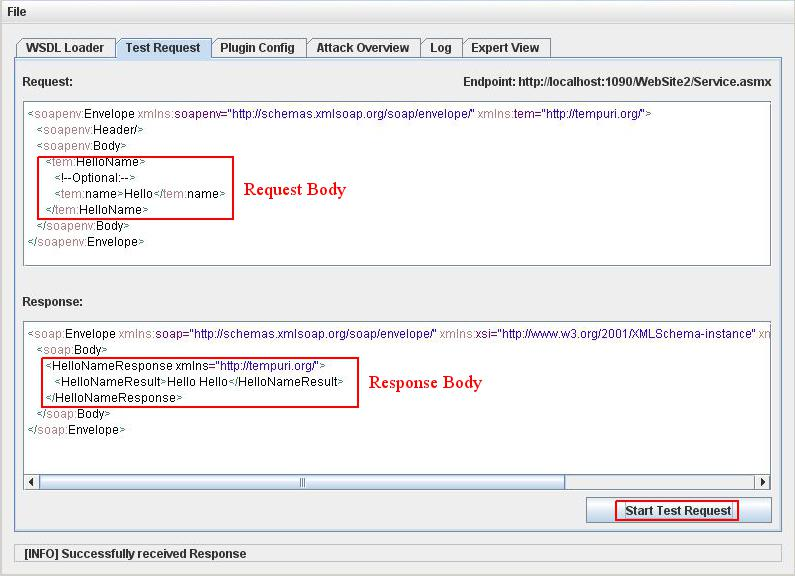
\includegraphics[width=0.8\textwidth]{img/test_request}
    \end{center}
    \caption{Submitting a test request.}
    \label{fig:test_request}
\end{figure}

\subsection{Attack Plugin Configuration}
\label{sec:attack_plugin_configuration}

The next step is to configure the plugins. In this case, the automatic mode is
used for SOAPAction Spoofing (Figure \ref{fig:plugin_config_sas}) and
the WS-Addressing Spoofing plugin detects the endpoint URL automatically
(Figure \ref{fig:plugin_config_wsas}), too -- there is nothing to
configure manually. The tree on the left shares different views on the plugins.
\emph{Active Plugins} contains all plugins which will be used for attacking the
server, \emph{All Plugins} contains all plugins ordered by their category and
\emph{Alphabetical Sorted} shows all plugins in an alphabetical order.

\begin{figure}[h!]
    \begin{center}
        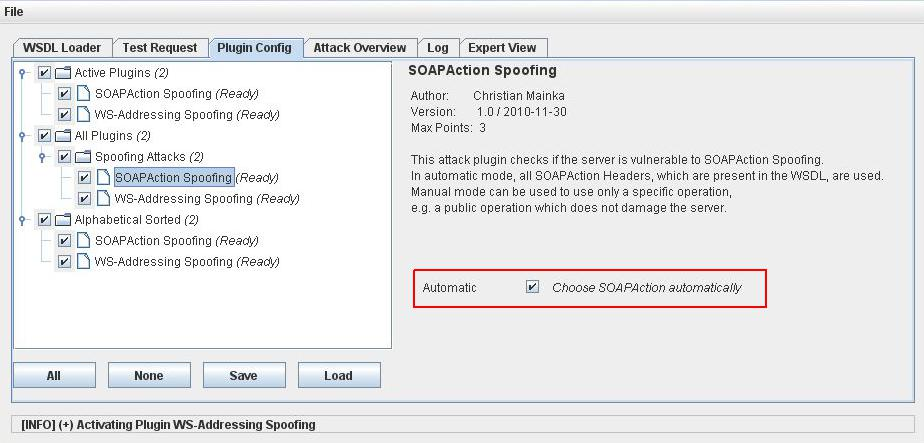
\includegraphics[width=0.8\textwidth]{img/plugin_config_sas}
    \end{center}
    \caption{Plugin configuration for SOAPAction Spoofing.}
    \label{fig:plugin_config_sas}
\end{figure}

\begin{figure}[h!]
    \begin{center}
        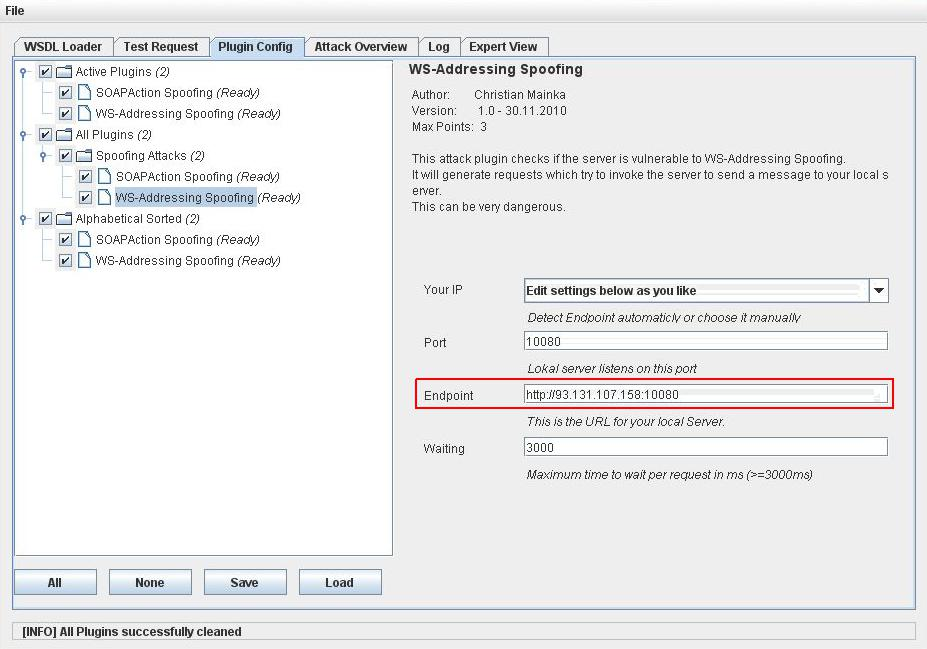
\includegraphics[width=0.8\textwidth]{img/plugin_config_wsas}
    \end{center}
    \caption{Plugin configuration for WS-Addressing Spoofing.}
    \label{fig:plugin_config_wsas}
\end{figure}

\subsection{Starting the Attacks}
\label{sec:starting_the_attacks}

The last step is to start the attack. Figure~\ref{fig:attack_done} shows
the overview of a finished attack run. Active plugins are displayed on the top,
their results at the bottom. The slider in the top part allows to filter the
results by their level. The user can choose to see only the most
\emph{important} results, or see even the request content at the \emph{tracing}
level.

\begin{figure}[h!]
    \begin{center}
        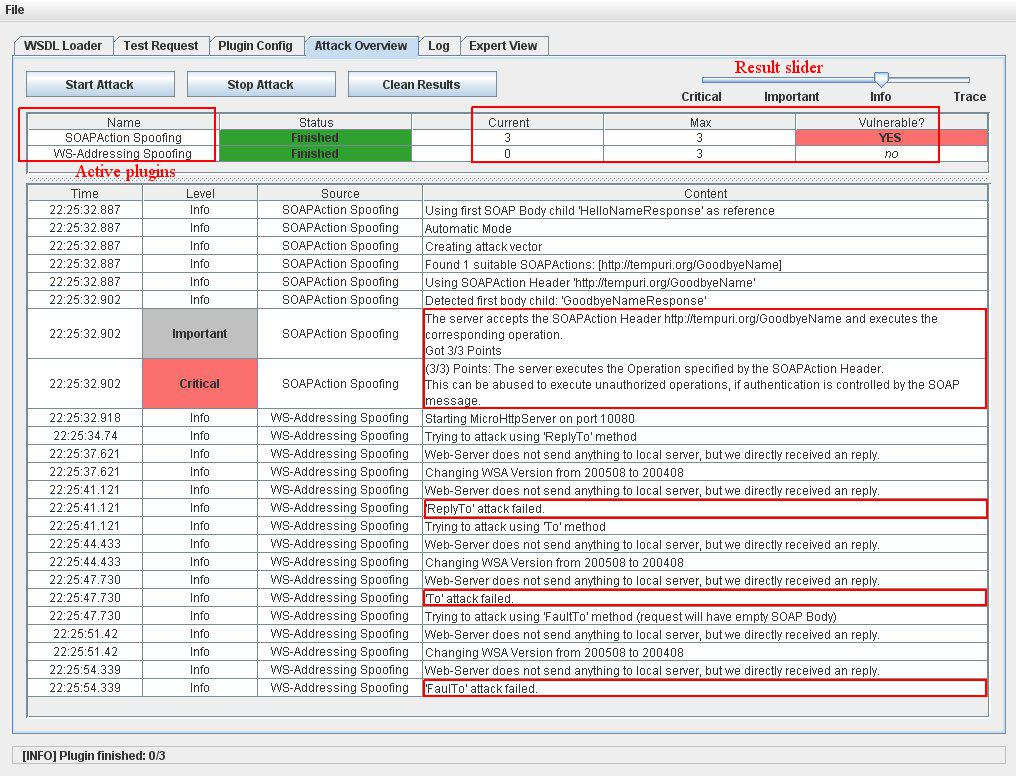
\includegraphics[width=0.8\textwidth]{img/attack_done}
    \end{center}
    \caption{Penetration test on .NET finished.}
    \label{fig:attack_done}
\end{figure}

The Web Service is vulnerable to SOAPAction Spoofing but resistant to
WS-Addressing Spoofing. This is indicated different aspects:

\begin{enumerate}
    \item The \emph{vulnerable} column values show \textbf{YES} for SOAPAction Spoofing and \emph{no} for WS-Addressing Spoofing.
    \item The SOAPAction Spoofing plugin got the maximum rating -- three of three points in this case -- and WS-Addressing Spoofing got zero points.
    \item The results show, that the server has executed the operation defined
        in the SOAPAction Header, which is the most critical security issue.
\end{enumerate}

\section{Automatic Detection of XML Signature Wrapping Attacks}
\label{sec:automatic_detection_of_xml_signature_wrapping_attacks}

\subsection{Introduction}
\label{sec:introduction}

XML Signature Wrapping (XSW) is a web service specific attack allows to modify signed
XML messages. 
It was firstly published in 2005 by McIntosh and Austel~\cite{xsw}. 
The basic idea of this attack is to trick out the reference mechanism which detects the signed parts
of an XML message and thus let it use a different message part than the application
logic uses.

The impact of this attack can be seen in~\cite{amazon} where the authors uses an XSW attack to
attack the Amazon EC21 and Eucalyptus2 SOAP interfaces. They only need to eavesdrop
a single SOAP message and afterwards, they are able to start, stop and download the
victims cloud instance.

In 2012, the authors have applied the attack technique to Single Sign-On scenarios and successfully attacked 11 out of 14 SAML frameworks, including Shiboleth and IBM DataPower~\cite{samlattacking}.

The WS-Attacker XSW Plugin and Library is mainly based on a Master Thesis by Christian Mainka\footnote{\url{http://nds.rub.de/media/nds/arbeiten/2012/07/24/ws-attacker-ma.pdf}}.

\subsection{Short Technical Attack Description}
\label{sec:short_technical_attack_description}

The most frequently used scenario for XML Signature is to refer the signed parts of an XML message by an ID attribute. 
This method is easy to understand for humans and simple to implement for developers. 
However, it has the big disadvantage that the signature itself only protects the content of the signed elements but not its location within the document. 
Thus, the signed element can be moved to another location -- vertically and horizontally in the Document structure -- without invalidating the signature. 

Figure~\ref{fig:xsw_id} gives an example for constructing an XSW message which still bypasses the signature verification process but changes the payload used by the application logic.

\begin{figure}[ht]
    \begin{center}
        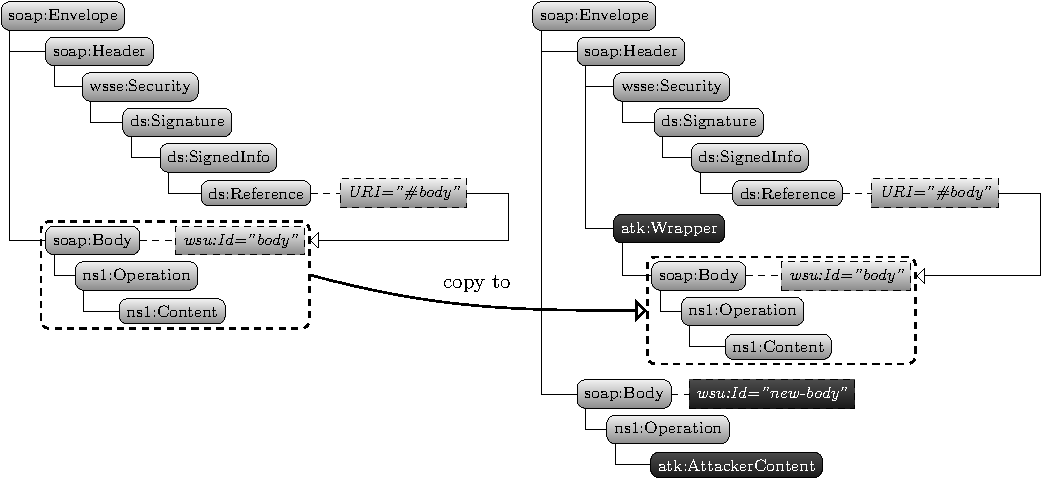
\includegraphics[width=\linewidth]{img/xsw_id}
    \end{center}
    \caption{Creating an XSW message for an ID referencing based XML Signature. 
The original signed message is shown on the left side.
The XSW message on the right side is constructed by copying the signed element to a \texttt{Wrapper} element and modifying the signed content to the attackers' needs.}
    \label{fig:xsw_id}
\end{figure}

The original message has a signed \texttt{Body} element which is referenced by the ID attribute \texttt{\#body}.
The attack message on the right has a new \texttt{Wrapper} element placed as a child of the \texttt{Header} element.
Its child is a copy of the original signed \texttt{Body} element.
Note that the ID attribute still has the value \texttt{\#body}.
The original \texttt{Content} element is replaced by a new \texttt{AttackerContent} element and the ID attribute of its ancestor \texttt{Body} element is changed to \texttt{new-body}, so that the signature verification logic will not use it.
There might also be other attack scenarios in which the attribute value remains the same as in the \texttt{Wrapper} element or it removed completely.
The success of this attack depends on the implemented application- and verification logic.

The main problem why this attack works is that the signature verification- and the application logic use different methods for detecting their elements.
The signature verification logic looks for an element which has the attribute \texttt{wsu:Id="body"} and uses it to compute the digest value.
The application logic, in contrast, does not care about the attribute \texttt{wsu:Id="body"} -- it just uses the first child element of the \texttt{Body} element in the SOAP message.
Obviously, these referencing methods are not equivalent, as the example attack message shows.

This is just the very basic example of one possible XSW techniques. More complicated attack variants can be found in~\cite{Liao2011},~\cite{2011:07:xmlSigConSAPSE} and the Master Thesis mentioned before.

\subsection{Using the XSW Plugin}
\label{sec:using_the_xsw_plugin}

This section will explain how to use the XSW plugin by an example attack on Apache Axis2 which uses the Rampart Security Module. 
For attacking the server, it is started with the policy example 02 distributed with Rampart. 

The first steps are similar to the common usage of WS-Attacker. 
You need to load the WSDL and choose the operation to attack. 
Afterwards you need a signed SOAP message to continue. 
Creating/Getting such messages can be a real challenge. 
One example to create such a message is to use SoapUI\footnote{\url{http://www.soapui.org/}}. 
However, this tool is only capable for creating ID based XML Signatures. 
Another example is using Wireshark4 and eavesdrop a message created by some client. 
For this scenario, the message created by the Rampart example client is eavesdropped. 

Next is to configure the plugin. Figure~\ref{fig:xsw_plugin_config} shows the configuration window.

\begin{figure}[ht]
    \begin{center}
        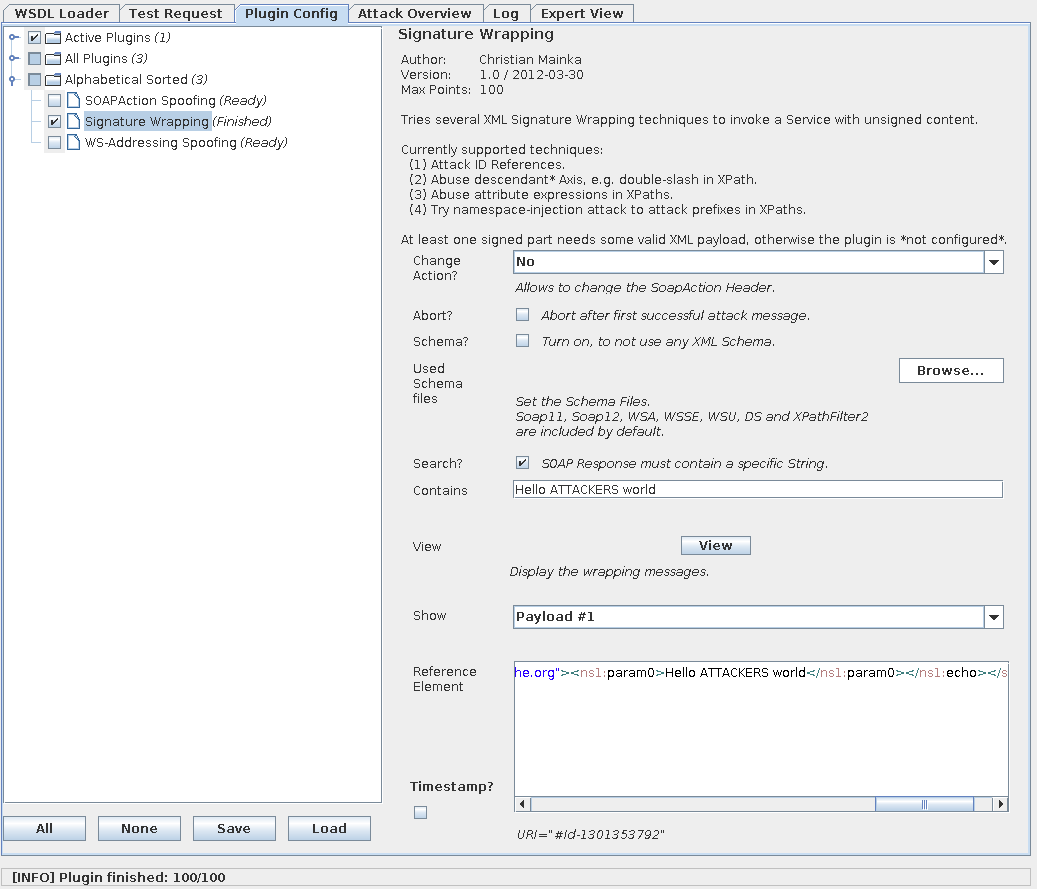
\includegraphics[width=0.9\linewidth]{img/xsw_attacking_axis_with_policy_config}
    \end{center}
    \caption{Configuration of the XSW plugin within the WS-Attacker framework.}
    \label{fig:xsw_plugin_config}
\end{figure}

\begin{itemize}
    \item It is possible to \textbf{change} the \textbf{SOAPAction} parameter. This can be useful if the attacker wants to invoke a different operation to the one he chose after loading the WSDL.
    \item If the \textbf{abort} checkbox is on, the attack will stop after the first successful attack. Otherwise, it will go on with further XSW messages. This can be usefull to detect more than one attack message.
    \item The \textbf{Schema Validation} can be optionally turned off. This might be useful if the server does not care on any XML Schema. However, the attack will be much slower as more XSW attack messages can be used.
    \item An optional \textbf{Search String} can be specified. This means, that each response, which is not a SOAP Fault, will be searched for this string. The attack is then only successful if the string is contained. This is useful to detect if the correct payload is used (in some cases, the original payload can be executed instead of the new one).
    \item A \textbf{view button} can be used to create and view all XSW messages without sending them to the server. If the WS-Attacker user knows the ID of the successful message (shown in log), he can use this button to re-create the message.
    \item The \textbf{dropdown} box must be used to set the payload. Note that the plugin is \textbf{not configured} if there is no payload set by the user.
\end{itemize}

After configuring the plugin, the attacks can be started as usual. An example result
window can be seen in Figure~\ref{fig:xsw_plugin_result}.

\begin{figure}[ht]
    \begin{center}
        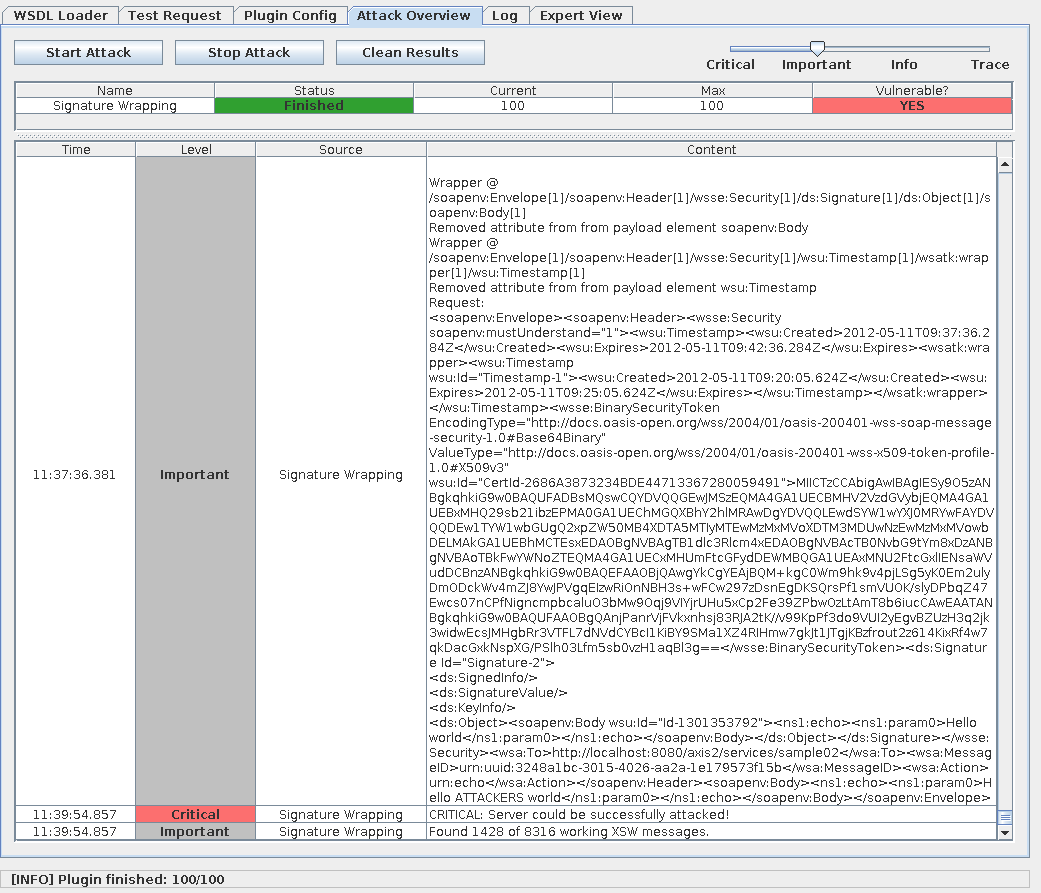
\includegraphics[width=0.9\linewidth]{img/xsw_attacking_axis_with_policy_result}
    \end{center}
    \caption{Results of the XSW plugin.}
    \label{fig:xsw_plugin_result}
\end{figure}

\section[DoS Extension]{How to Use the DoS Extension of the WS-Attacker}
\label{sec:how_to_use_dos_extension}

This guide shows how to use the DoS attack plugins of the WS-Attacker.

\subsection{General Design of the WS-Attacker DoS Extension}
\label{sec:design_DoS_extension}

The design of the automated Web service DoS attack tool is shown in Figure~\ref{fig:architectureDosAttackTool} using a UML-based activity diagram to describe the high level program flow.
This newly created design is especially tailored towards solving the problems caused by using the blackbox approach when measuring the attack success.\newline

For each Web service specific DoS attack, the following nine parameters have to be set up:
\begin{itemize}
  \item M = number of sequential (un)tampered requests per thread 
  \item N = number of parallel threads 
  \item T = milliseconds between continuous untampered testprobe requests
  \item K = milliseconds between each (un)tampered request 
  \item X = seconds between receiving last untampered request and sending first untampered request 
  \item S = seconds between receiving last tampered request and finalization (end) of the attack 
  \item L = number of network stability test requests
  \item R = milliseconds between each network stability test request 
  \item Message = the string will be used to create a tampered request.\\
  By default, this variable holds the original SOAP request of the targeted Web service.\\
  The string value can be set to an arbitrary value. No valid XML is required.\\
  If set by the attack developer, the string can hold a payload placeholder. This allows a tester to place the payload to the position required for the attack to work.
\end{itemize}

\newpage
Furthermore, the following two boolean values have to be set: 
\begin{itemize}
  \item Boolean attackStop\\If true, the attack will finalize automatically after S seconds. Otherwise, the attack will run until the user finalizes the attack manually. 
  \item Boolean performNetworkStabilityTest\\If true, network stability test will get performed. Otherwise, it will get skipped.
\end{itemize}

The program flow when executing a single attack is shown in Figure~\ref{fig:architectureDosAttackTool}.
\begin{landscape}
  \begin{figure}[!ht]
	  \centering
	  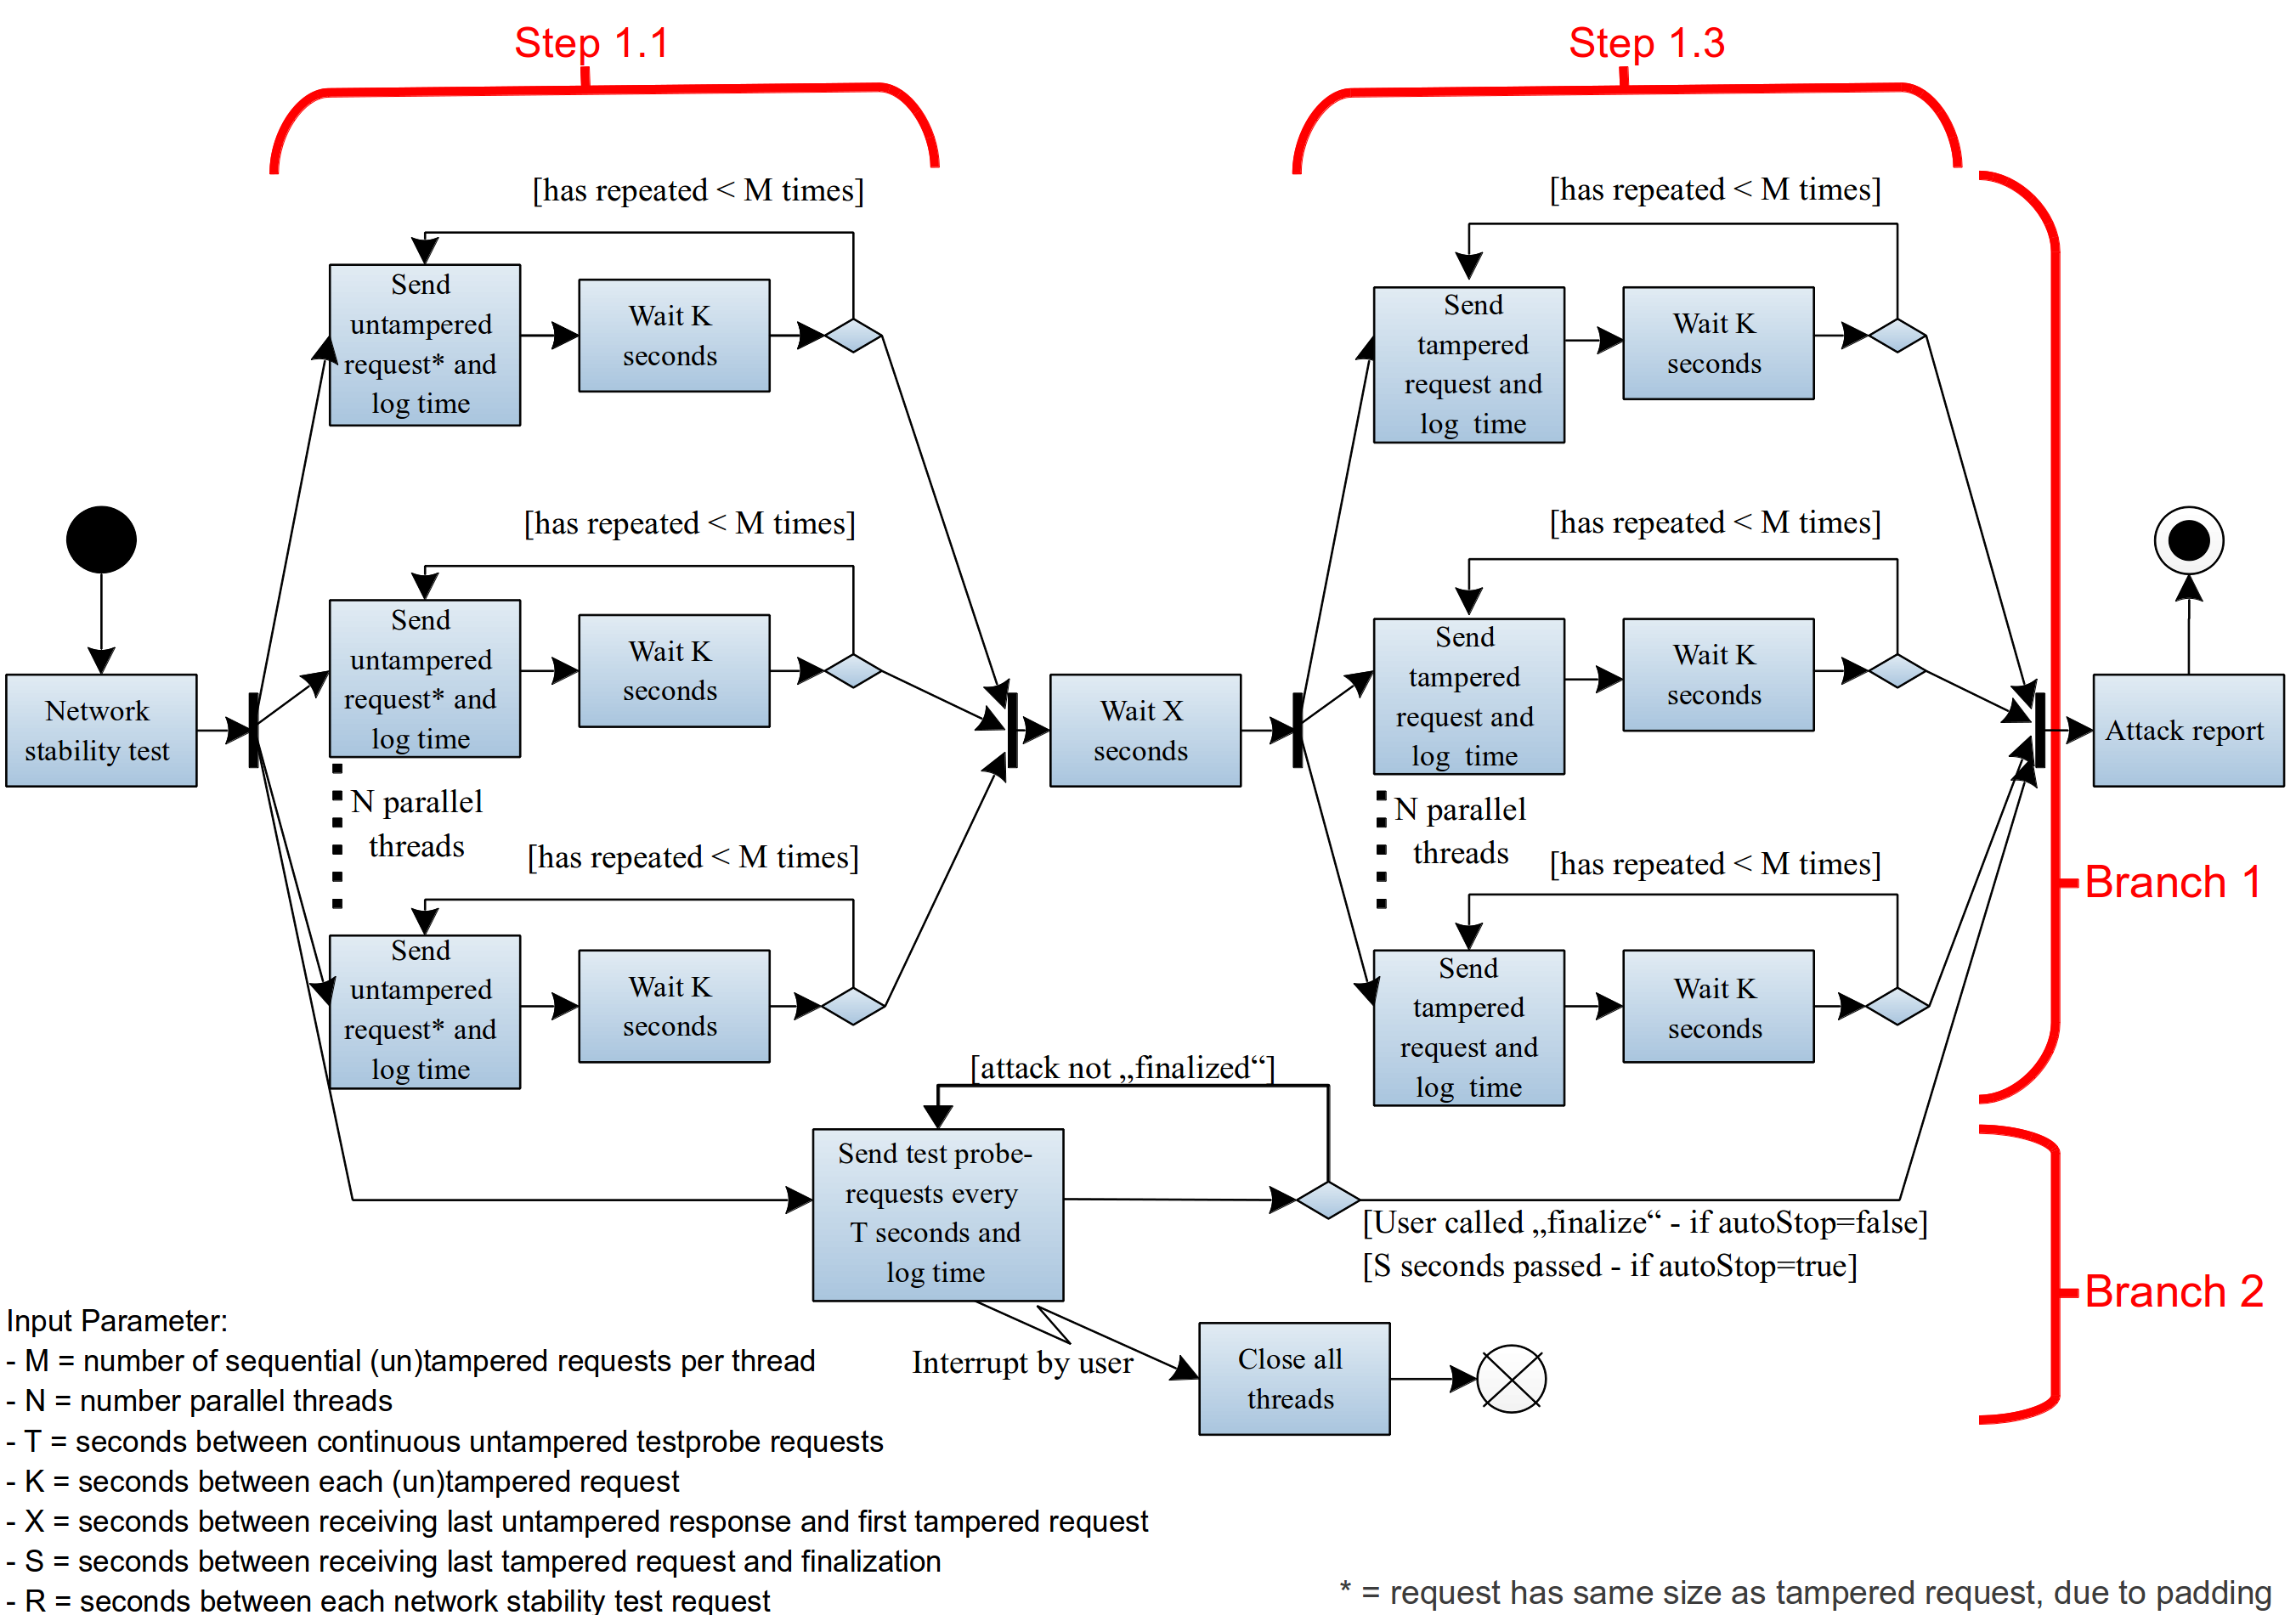
\includegraphics[width=21cm]{img/architecture.png}
	  \caption{Architecture of an automated Web service specific DoS attack tool}
	  \label{fig:architectureDosAttackTool}
  \end{figure}
\end{landscape}

The steps in Figure~\ref{fig:architectureDosAttackTool} are as follows:
  \begin{enumerate}
    \item Test network stability\par When the program is started, a network stability test will get performed (only when enabled by the user). The outcome will tell the tester whether or not a penetration test is feasible under the given network delays. The result has just informative character. A negative result of the network stability test will not stop the program. 
    \item Perform attack\par After the network stability test, the program flow splits into two branches.  
    \begin{enumerate}
      \item Branch 1: Perform attack including error correction\par This branch performs the actual attack. However, errors might occur. Therefore, branch 1 is split into three substeps.
      \begin{enumerate}
	\item Branch 1 - step 1:\\Open N threads in parallel and send M untampered requests per thread.\par Each thread induces a delay of K seconds between each request. The delay timer starts as soon as the the client tries to send the request. It is not waited until a response is returned. Otherwise, reproducible results would not be possible.
	\item Branch 1 - step 2:\\Wait for X seconds. 
	\item Branch 1 - step 3:\\Open N threads in parallel and send M tampered requests per thread.\par Each thread induces a delay of K seconds between each request.
      \end{enumerate}  
      \item Branch 2: Simulate regular user who uses the Web service while attack is running\par Branch 2 continuously sends untampered requests to the Web service with a delay of T seconds between each request. This process continues until the attack is finalized.  The attack finalization can be triggered by the user if the boolean attackStop is set to false. Otherwise, the attack will stop automatically after S seconds.
    \end{enumerate}
    \item Attack results\par Branch 1 and branch 2 are finished. All logged data is grouped and analyzed by the program. Each logged request will get assigned to an discrete interval. By default the interval length is one second. 
    The attack results will be presented in the attack report. Options for saving the results are also presented.
  \end{enumerate}


This software design was newly created; incorporating the goal of creating a fully automated Web service specific DoS attack tool using the blackbox approach. 
The design meets the following requirements:

\minisec{Automated Crafting and Sending of Attack Messages for Chosen DoS Attack}
\label{sec:ImpAutomatedSending}
All requests are created by the DoS attack tool.
Based on the chosen attack parameters, the requests get sent automatically for the defined number of times. 

\minisec{Fitness for Various Load Scenarios}
\label{sec:ImpLoadScenario}
By setting up the parameters 
\begin{enumerate}
  \item M = number of sequential (un)tampered requests per thread 
  \item N = number parallel threads 
  \item K = milliseconds between each (un)tampered request
\end{enumerate}
the penetration tester is able to define arbitrary load scenarios. 

\minisec{Fitness for Various Test Scenarios}
\label{sec:ImpTestScenarios}
The design shown in Figure \ref{fig:architectureDosAttackTool} allows for testing of two distinct test scenarios. 
\begin{enumerate}
  \item Test for vulnerability.\\
  A vulnerability test can be conducted by running an attack with very few requests.
  Ideally, one thread with one request is enough to decide whether or not the target is vulnerable to the chosen Dos attack.
  
  \item Test for attack effect on third party users.\\
  A test that checks if third party users are affected can be achieved by increasing the duration of the attack and the load per interval. 
  There is no default option provided for this test scenario. The hardware performance of the tested system can vary heavily. 
  Therefore, a tester has to manually vary the parameters and rerun the test until the desired result is achieved on a vulnerable system.\\
\end{enumerate}

\minisec{Elimination of Errors}
\label{sec:ImpErrors}
Elimination of the errors takes place in branch 1 of the activity diagram. 
Step 1.1 and step 1.3 both cause the same load on the network:
\begin{itemize}
 \item The time pattern in which the messages are sent is equal.
 \item The message size of untampered and tampered requests is equal, due to message padding.
\end{itemize}
The only difference between these steps is that step 1.1 sends untampered requests and step 1.3 sends tampered requests.  
When using this pattern, any significant difference in roundtrip time between tampered and untampered requests must be caused by the attack payload.\\

\minisec{Exclusion of Subattacks}
Some attacks are composed of different subattacks. However, a tester might want to test for only one of the subattacks. 
In this case, the tampered request has to hold the payload of the entire attack. The untampered request has to hold the payload of the subattacks the tester doesn’t want to test for. 
When calculating the attack success metric, only the impact of the subattack that is not included in the untampered request is considered.



\subsection{Walktrough example of a coercive Parsing Attack}
\label{sec:walkthrough_example}

In the following a full attack walkthrough of a coercive parsing DoS vulnerability test is given. Information on the coercive parsing attack can be found here: \url{http://ws-attacks.org/index.php/Coercive_Parsing}
The general steps required to perform a DoS vulnerability test are as follows: 
\begin{enumerate}
    \item Load the WSDL.
    \item Submit a test request.
    \item Select and configure the ``coercive parsing'' attack plugin.
    \item Start the attack.
    \item View attack results.
\end{enumerate}

The steps needed to run any other DoS attack plugin are similar. 
Only in step 3 slight differences can occur, since the attack specific parameters might vary based on the chosen attack.


\subsubsection{Load the WSDL}
\label{sec:loading_a_wsdl_dos}

After starting WS-Attacker, the GUI appears and offers an input field to enter the location
of the WSDL, see Figure \ref{fig:dosStep1}.

\begin{figure}[h!]
    \begin{center}
        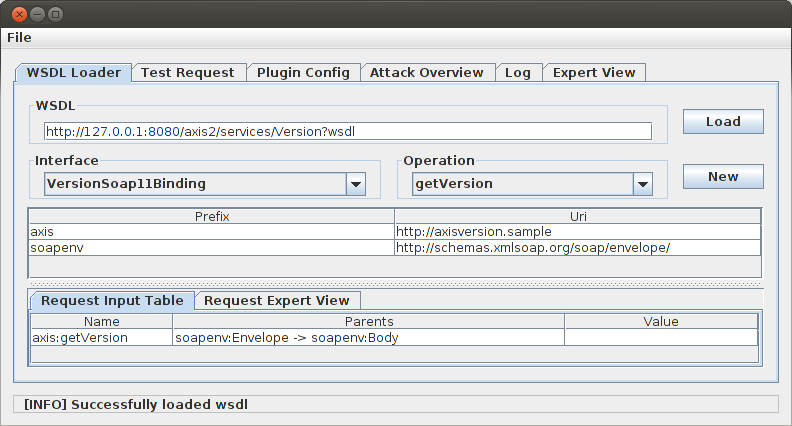
\includegraphics[width=0.8\textwidth]{img/dosStep1}
    \end{center}
    \caption{Loading the WSDL.}
    \label{fig:dosStep1}
\end{figure}

In this testcase the WSDL file \url{http://127.0.0.1:8080/axis2/services/Version?wsdl} is loaded. All other parameters are left at their default values. 
For more information on the other parameters please refer to the general WS-Attacker documentation.

\subsubsection{Submit a test request}
\label{sec:submitting_a_test_request_dos}
Next step is to do a test request: Figure \ref{fig:dosStep2} shows
the test request and the corresponding response. 
The test request is very important. It is used as the baseline request for all further testing. 
Based on this test request, all attack payloads will be build later on.

\begin{figure}[h!]
    \begin{center}
        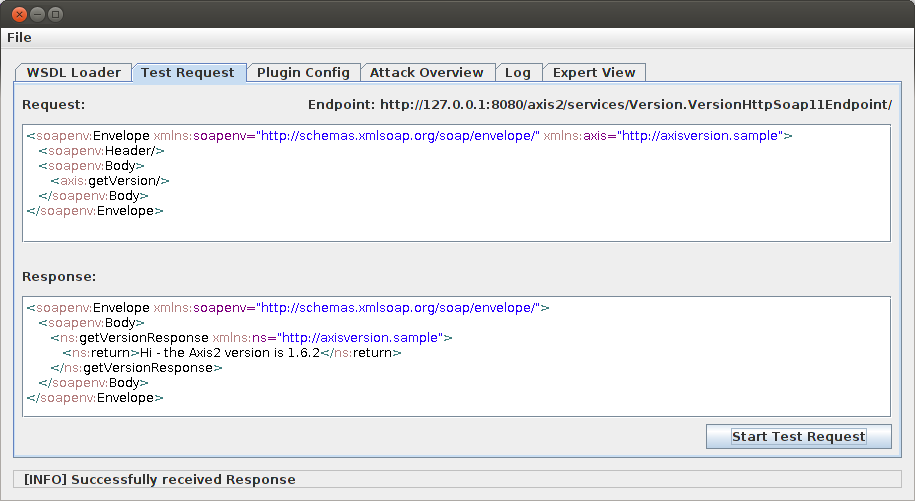
\includegraphics[width=0.8\textwidth]{img//dosStep2}
    \end{center}
    \caption{Submitting a test request.}
    \label{fig:dosStep2}
\end{figure}

\subsubsection{Select and configure the attack plugins}
\label{sec:attack_plugin_configuration_dos}

Next the attack plugin is selected and configured. In this scenario, only the coercive parsing DoS attack
is chosen. As soon as the plugin is selected, the attack options will show up on the right side (Figure \ref{fig:dosStep3}). 

\begin{figure}[H]
    \begin{center}
        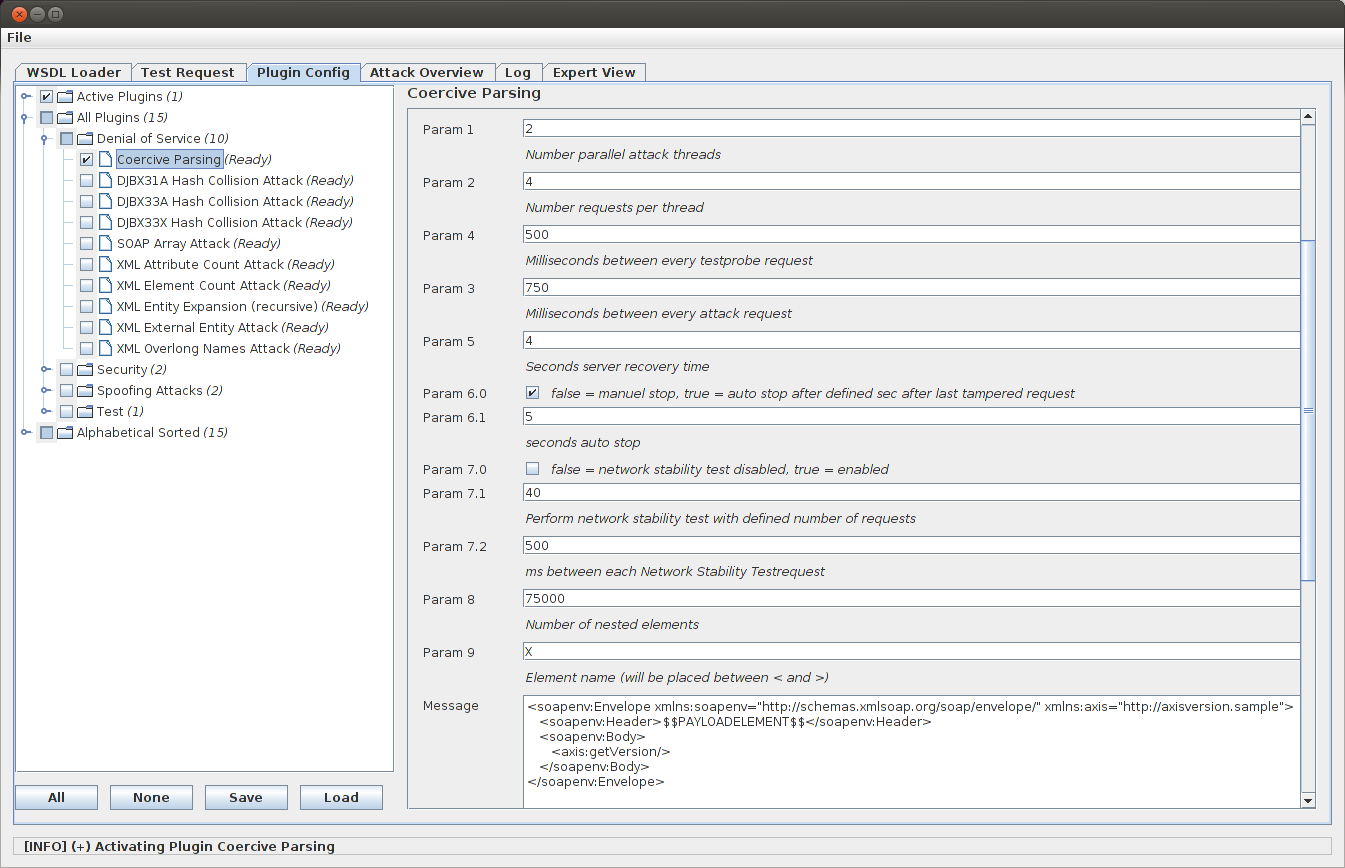
\includegraphics[width=0.95\textwidth]{img/dosStep3_1.png}
    \end{center}
    \caption{Selected attack plugin ``coercive parsing''}
    \label{fig:dosStep3}
\end{figure}

In general the DoS attack plugin can be left at its default parameters. 
Any vulnerable Web Service should be clearly marked as vulnerbale with the default parameters. 

The plugin offers the following attack specific options:
\begin{itemize}
    \item Number of nested elements \\The default number is at 75000. This means 75000 XML elments will be nested within each other.
    \item Element name (will be placed between < and >) \\The default element name is ''x``.
\end{itemize}

The following DoS attack extension specific parameters can be left unchanged:
\begin{itemize}
    \item Number parallel attack threads
    \item Number requests per thread 
    \item Milliseconds between every testprobe request
    \item Milliseconds between every attack request
    \item Seconds server recovery time
    \item Auto stop switch
    \item seconds auto stop
    \item Network stability test 
    \item Perform network stability test with defined number of requests
    \item Ms between each Network Stability Testrequest
    \item Message
\end{itemize}

\subsubsection{Start the attack}
\label{sec:starting_the_attacks_dos}

The last step is to start the attack. 
Just switch to the \"Attack Overview\"-tab and press the start button. See Figure~\ref{fig:dosStep4}.

\begin{figure}[H]
    \begin{center}
        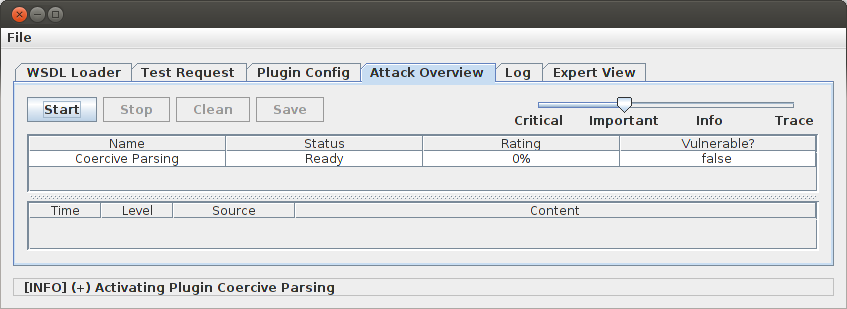
\includegraphics[width=0.95\textwidth]{img/dosStep4.png}
    \end{center}
    \caption{Starting the attack.}
    \label{fig:dosStep4}
\end{figure}

While the attack is running
\begin{figure}[H]
    \begin{center}
        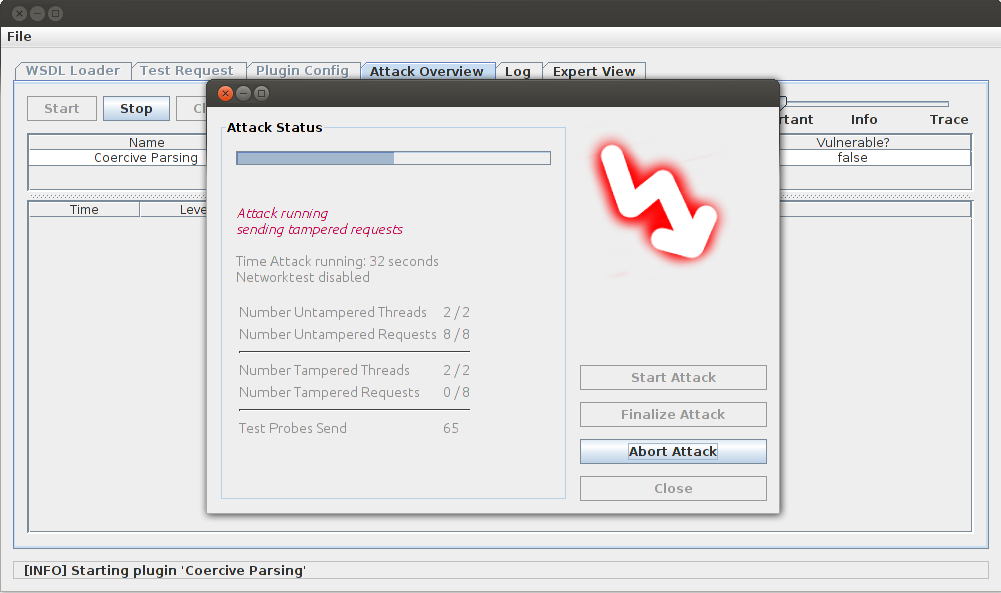
\includegraphics[width=0.8\textwidth]{img/dosStep4_1.png}
    \end{center}
    \caption{Attack is running}
    \label{fig:dosStep4_1}
\end{figure}


\subsubsection{View attack results}
\label{sec:view_results}

Once the attack is finished, the status column should turn green. The column ''Rating`` and ''vulnerable`` already give a rough hint of the attack success.
As shown in Figure~\ref{fig:dosStep4_2}, the tested Web Service is rated as 100\% vulnerbale. 
\begin{figure}[ht!]
    \begin{center}
        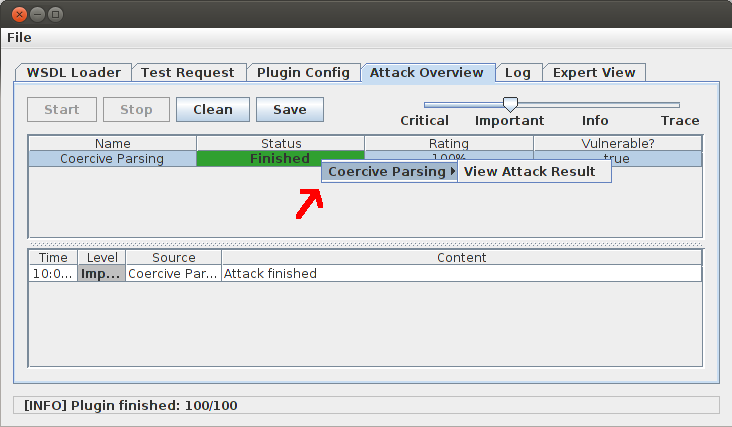
\includegraphics[width=0.95\textwidth]{img/dosStep4_2.png}
    \end{center}
    \caption{Penetration test finished}
    \label{fig:dosStep4_2}
\end{figure}

In Order to see a detailed attack description, just right click the coercive parsing attack row. 
A sub menu will show that lets you choose the ''View Attack Results`` option. The final attack result are presented in Figure~\ref{fig:dosStep4_3}.
\begin{figure}[H]
    \begin{center}
        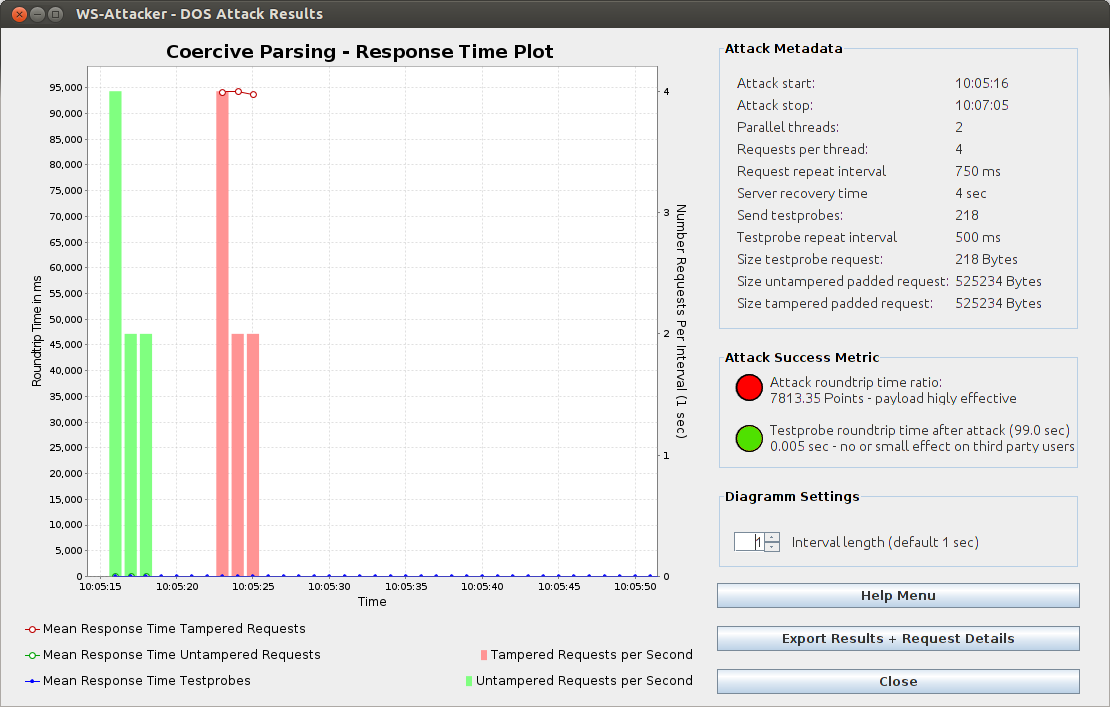
\includegraphics[width=0.95\textwidth]{img/dosStep4_3.png}
    \end{center}
    \caption{View attack result details}
    \label{fig:dosStep4_3}
\end{figure}
As shown in Figure~\ref{fig:dosStep4_3}, the tested Web Service is clearly vulnerable. 
The ''attack roundtrip time ratio`` is at 7813. This means that on average, the response time of a tampered request is 7813 times longer than a regular untampered request under the same load scenario.

The attack results with all details (including all payload requests) can be saved as Txt-File and Jpg-File by clicking the button ''Export Results + Request Details``.
A new instance of Firefox should pop up that provides links to the result files.

XML Encryption is a W3C standard used for encryption of XML documents~\cite{Eastlake2013}. It is typically used in Web Services applications or for encryption of SAML tokens in Single Sign-On scenarios.

XML Encryption defines (among others) two cryptographic algorithms: RSA PKCS\#1 v1.5 and AES/3DES in CBC (Cipher Block Chaining) mode of operation. These two algorithms are vulnerable to so called adaptive chosen-ciphertext attacks, which has been shown in many practical examples. Thus, it is not surprising that XML Encryption applications were also found to be vulnerable to those attacks:

\begin{itemize}
 \item In 2011, we presented a paper on How to Break XML Encryption~\cite{CCS:JagSom11}, which showed how to attack symmetric key encryption algorithms in CBC mode. The idea is very similar to the typical padding oracle attacks, it is just a slightly more complicated, since we use XML parsing errors as a side-channel. A very good summary on this attack gives Matthew Green.\footnote{\url{http://blog.cryptographyengineering.com/2011/10/attack-of-week-xml-encryption.html}}
 \item In 2012, we showed how to apply Bleichenbacher's attack on the asymmetric encryption algorithm (RSA PKCS#1) in XML Encryption~\cite{ESORICS:JagSchSom12}. A summary on Bleichenbacher's attack is given on our blog.\footnote{\url{http://web-in-security.blogspot.de/2014/08/old-attacks-on-new-tls-implementations.html}}
\end{itemize}

    
    

All you need to know for now is that both attacks belong to the family of adaptive chosen ciphertext attacks.

\begin{figure}[ht]
    \begin{center}
        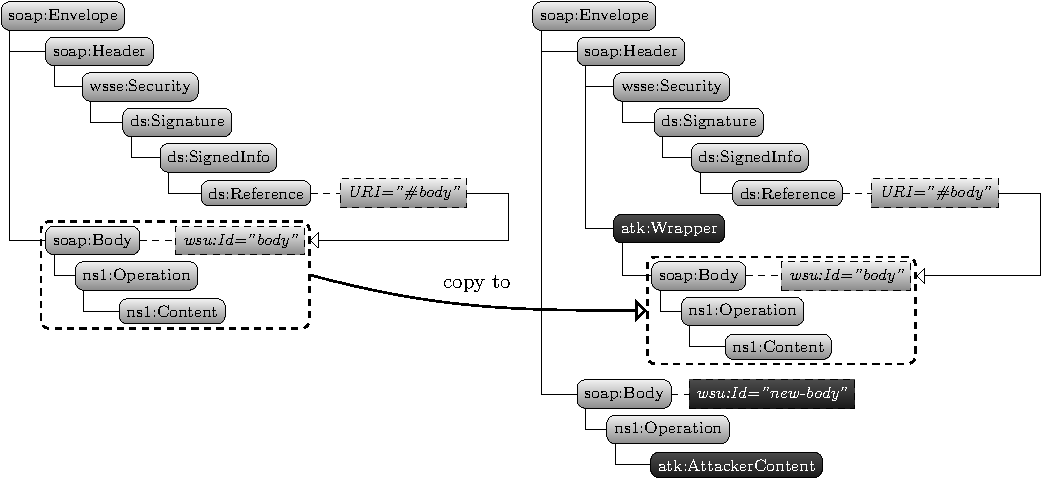
\includegraphics[width=\linewidth]{img/xsw_id}
    \end{center}
    \caption{Creating an XSW message for an ID referencing based XML Signature. 
The original signed message is shown on the left side.
The XSW message on the right side is constructed by copying the signed element to a \texttt{Wrapper} element and modifying the signed content to the attackers' needs.}
    \label{fig:xsw_id}
\end{figure}

The attacker, who eavesdrops an encrypted message, uses the message receiver as an oracle. He sends to the oracle modified ciphertexts and observes its response (it can contain a general error, a parsing failure, or just a valid response text). Based on the responses, he learns the plaintext.

\appendix
\addcontentsline{toc}{section}{Appendix}
\section*{Appendix}
\ohead[]{Appendix}
\ihead[]{}
\let\section\subsection
% \selectbiblanguage{english}
\bibliography{literature}
\bibliographystyle{unsrtnat}

\end{document}
